% !TEX root = thesis.tex

%%
%%
%% results tables and figures appendix
%%
%%

%%
%% Section
%%
\section{Uniform risk on a uniform population}

%%
%% Tables and figures for uniform population of 10,000, uniform intensity of factor 50
%%
\graphicspath{{./results/unif_50_unif/}}
\makeatletter
\def\input@path{{./results/unif_50_unif/}}
\makeatother

\begin{table}[H]
        \centering
    \scriptsize

    \begin{subtable}{0.5\textwidth}
    \subcaption{Means} 
    % latex table generated in R 3.3.3 by xtable 1.8-2 package
% Mon Jan 15 21:47:29 2018
\begin{tabular}{lrrr}
  \hline
 & Oracle & Silverman & CV \\ 
  \hline
MISE & 0.000022 & 0.000035 & 0.000033 \\ 
  Relative MISE & 0.003402 & 0.005404 & 0.004996 \\ 
  Normalized MISE & 0.000022 & 0.000035 & 0.000033 \\ 
  MIAE & 0.002515 & 0.003126 & 0.003003 \\ 
  Relative MIAE & 0.031137 & 0.038695 & 0.037178 \\ 
  Max Error & 0.021087 & 0.031111 & 0.029319 \\ 
  Peak bias & -0.010671 & 0.006739 & 0.004427 \\ 
  Relative Peak bias & -0.132093 & 0.083426 & 0.054803 \\ 
  Peak drift & 0.288634 & 0.418493 & 0.401299 \\ 
  Relative Peak drift & 0.041233 & 0.059785 & 0.057328 \\ 
  Centroid bias & -0.011216 & -0.000155 & -0.001331 \\ 
  Relative Centroid bias & -0.138849 & -0.001917 & -0.016472 \\ 
  Centroid drift & 0.207657 & 0.222708 & 0.221023 \\ 
  Relative Centroid drift & 0.029665 & 0.031815 & 0.031575 \\ 
   \hline
\end{tabular}

    \end{subtable}%
    \begin{subtable}{0.5\textwidth}
    \subcaption{Standard deviations} 
    % latex table generated in R 3.4.2 by xtable 1.8-2 package
% Thu Feb 15 19:57:40 2018
\begin{tabular}{lrrr}
  \hline
 & Oracle & Silverman & CV \\ 
  \hline
MISE & 0.000089 & 0.000116 & 0.000228 \\ 
  Relative MISE & 0.000131 & 0.000171 & 0.000335 \\ 
  Normalized MISE & 0.000018 & 0.000023 & 0.000046 \\ 
  MIAE & 0.000911 & 0.000820 & 0.001681 \\ 
  Relative MIAE & 0.001105 & 0.000994 & 0.002040 \\ 
  Max Error & 0.024919 & 0.036302 & 0.058950 \\ 
  Peak bias & 0.031372 & 0.045576 & 0.062499 \\ 
  Relative Peak bias & 0.038067 & 0.055302 & 0.075836 \\ 
  Peak drift & 0.060193 & 0.086240 & 0.111909 \\ 
  Relative Peak drift & 0.008599 & 0.012320 & 0.015987 \\ 
  Centroid bias & 0.031457 & 0.047196 & 0.046071 \\ 
  Relative Centroid bias & 0.038170 & 0.057267 & 0.055902 \\ 
  Centroid drift & 0.051758 & 0.054538 & 0.052729 \\ 
  Relative Centroid drift & 0.007394 & 0.007791 & 0.007533 \\ 
   \hline
\end{tabular}

    \end{subtable}

    \caption[]{Error rates for uniform population of 10,000, uniform intensity of factor 50}
    \label{tbl:mean_error_rates:unif_50_unif}
\end{table}

\begin{figure}[H]
        \centering
    \begin{subfigure}[t]{0.32\textwidth}
    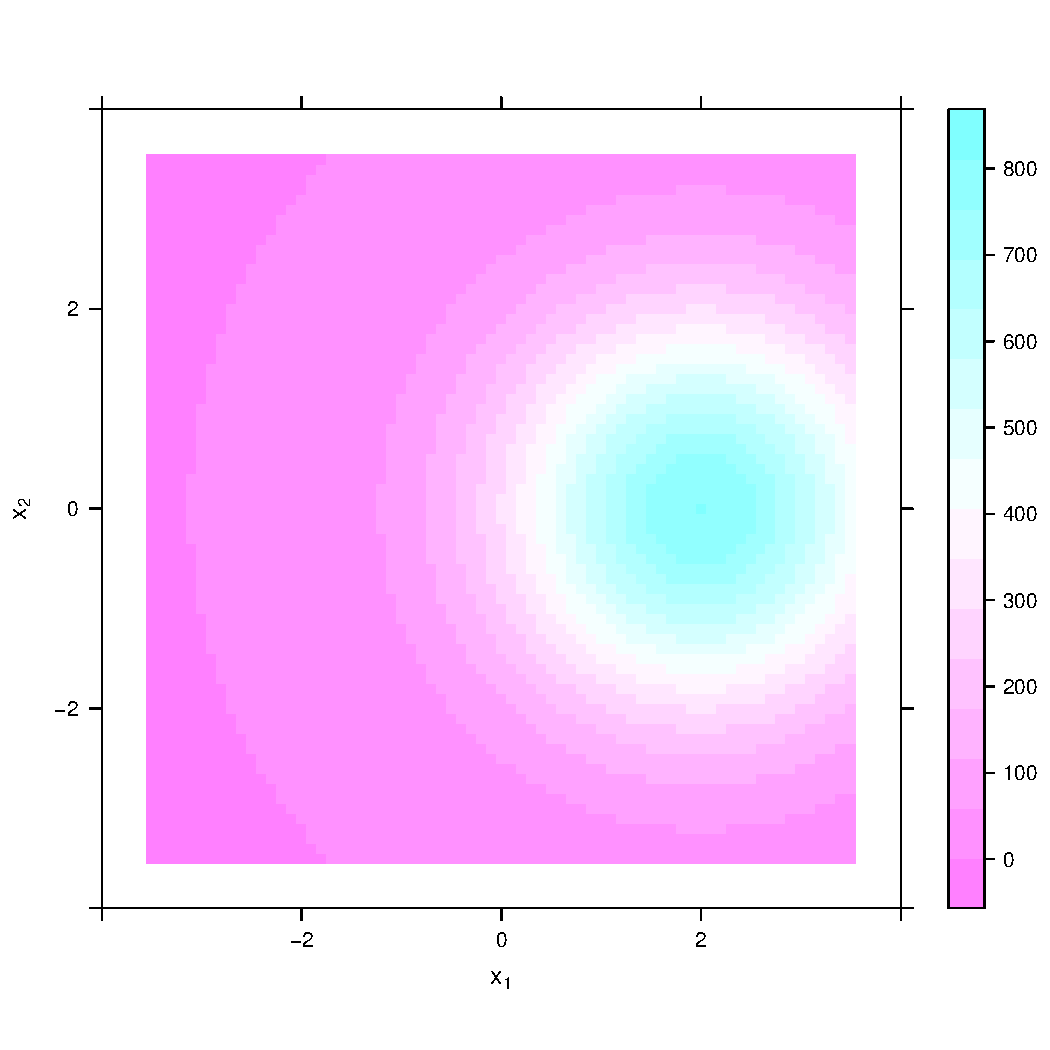
\includegraphics[width=\textwidth]{output/population-heatmap}
    \subcaption{Population distribution}
    \end{subfigure}
    \begin{subfigure}[t]{0.32\textwidth}
    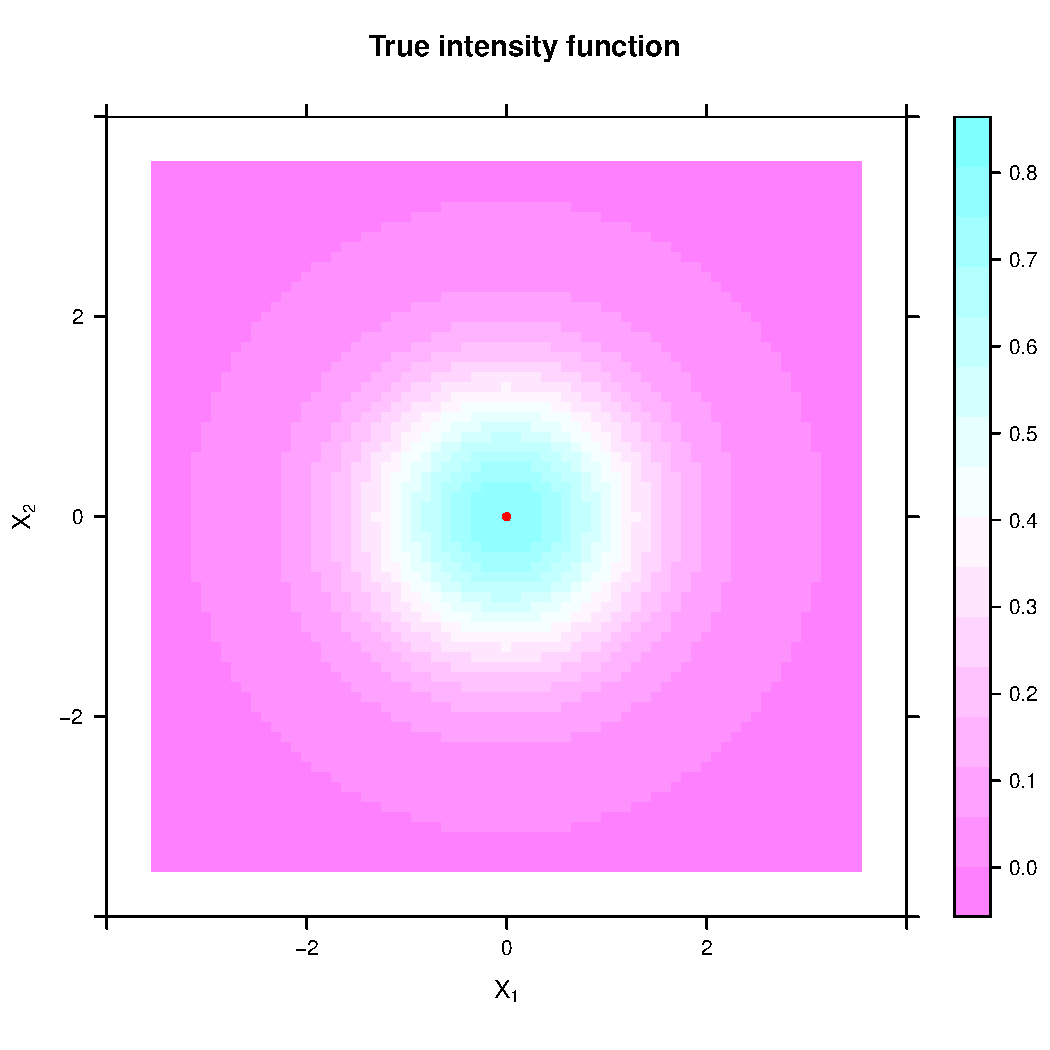
\includegraphics[width=\textwidth]{output/true_intensity_heatmap}
    \subcaption{True risk function}
    \end{subfigure}%
    \begin{subfigure}[t]{0.32\textwidth}
    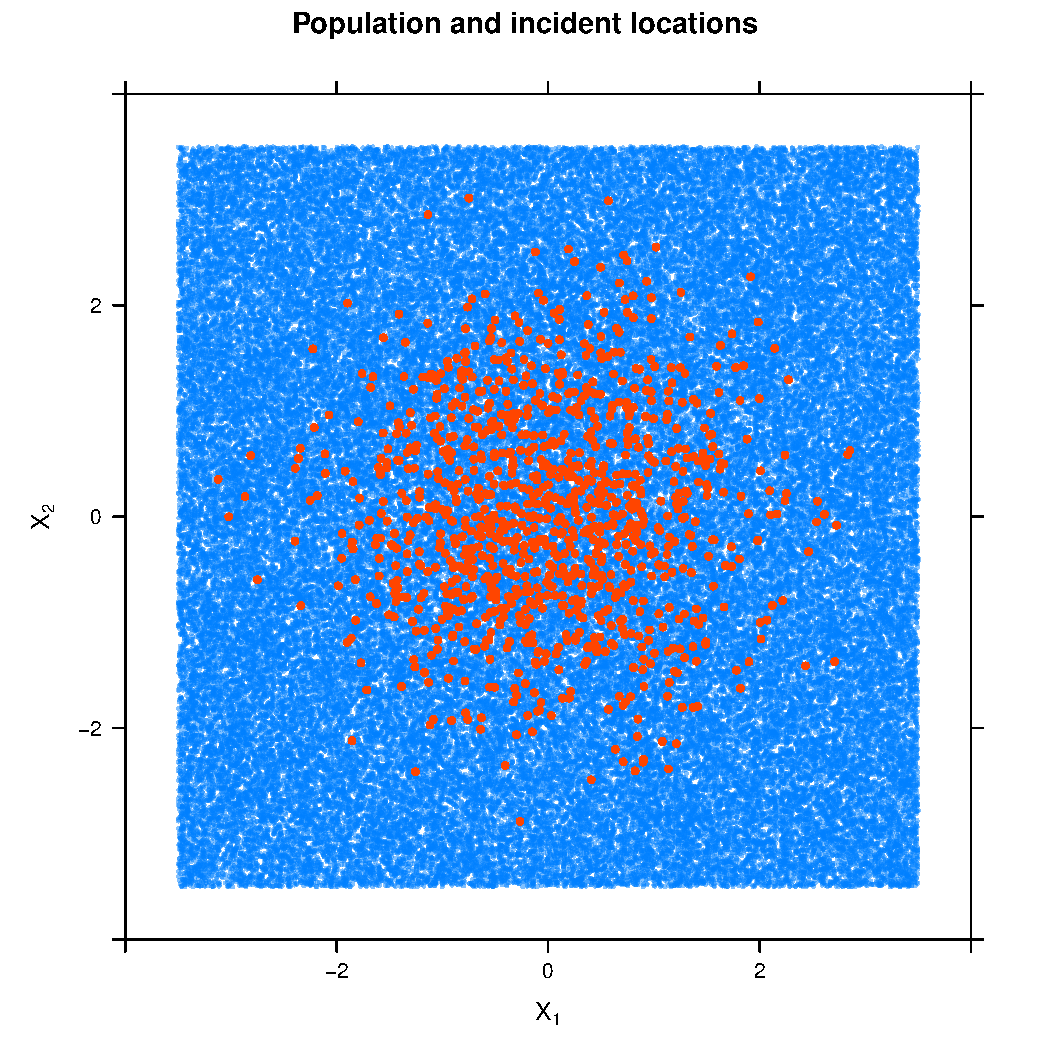
\includegraphics[width=\textwidth]{output/population_and_incidents_scatter}
    \subcaption{Population points (blue) with incidents (red)}
    \end{subfigure}%

    \caption[]{Population distribution (a), true risk function (b), and sample population with incidents (c) for uniform population of 10,000, uniform intensity of factor 50}
    \label{fig:distributions:unif_50_unif}    
\end{figure}


%%
%% Tables and figures for uniform population of 10,000, uniform intensity of factor 100
%%
\graphicspath{{./results/unif_100_unif/}}
\makeatletter
\def\input@path{{./results/unif_100_unif/}}
\makeatother

\begin{table}[H]
    \centering
    \scriptsize

    \begin{subtable}{0.5\textwidth}
    \subcaption{Means} 
    % latex table generated in R 3.3.3 by xtable 1.8-2 package
% Mon Jan 15 21:47:29 2018
\begin{tabular}{lrrr}
  \hline
 & Oracle & Silverman & CV \\ 
  \hline
MISE & 0.000022 & 0.000035 & 0.000033 \\ 
  Relative MISE & 0.003402 & 0.005404 & 0.004996 \\ 
  Normalized MISE & 0.000022 & 0.000035 & 0.000033 \\ 
  MIAE & 0.002515 & 0.003126 & 0.003003 \\ 
  Relative MIAE & 0.031137 & 0.038695 & 0.037178 \\ 
  Max Error & 0.021087 & 0.031111 & 0.029319 \\ 
  Peak bias & -0.010671 & 0.006739 & 0.004427 \\ 
  Relative Peak bias & -0.132093 & 0.083426 & 0.054803 \\ 
  Peak drift & 0.288634 & 0.418493 & 0.401299 \\ 
  Relative Peak drift & 0.041233 & 0.059785 & 0.057328 \\ 
  Centroid bias & -0.011216 & -0.000155 & -0.001331 \\ 
  Relative Centroid bias & -0.138849 & -0.001917 & -0.016472 \\ 
  Centroid drift & 0.207657 & 0.222708 & 0.221023 \\ 
  Relative Centroid drift & 0.029665 & 0.031815 & 0.031575 \\ 
   \hline
\end{tabular}

    \end{subtable}%
    \begin{subtable}{0.5\textwidth}
    \subcaption{Standard deviations} 
    % latex table generated in R 3.4.2 by xtable 1.8-2 package
% Thu Feb 15 19:57:40 2018
\begin{tabular}{lrrr}
  \hline
 & Oracle & Silverman & CV \\ 
  \hline
MISE & 0.000089 & 0.000116 & 0.000228 \\ 
  Relative MISE & 0.000131 & 0.000171 & 0.000335 \\ 
  Normalized MISE & 0.000018 & 0.000023 & 0.000046 \\ 
  MIAE & 0.000911 & 0.000820 & 0.001681 \\ 
  Relative MIAE & 0.001105 & 0.000994 & 0.002040 \\ 
  Max Error & 0.024919 & 0.036302 & 0.058950 \\ 
  Peak bias & 0.031372 & 0.045576 & 0.062499 \\ 
  Relative Peak bias & 0.038067 & 0.055302 & 0.075836 \\ 
  Peak drift & 0.060193 & 0.086240 & 0.111909 \\ 
  Relative Peak drift & 0.008599 & 0.012320 & 0.015987 \\ 
  Centroid bias & 0.031457 & 0.047196 & 0.046071 \\ 
  Relative Centroid bias & 0.038170 & 0.057267 & 0.055902 \\ 
  Centroid drift & 0.051758 & 0.054538 & 0.052729 \\ 
  Relative Centroid drift & 0.007394 & 0.007791 & 0.007533 \\ 
   \hline
\end{tabular}

    \end{subtable}

\caption[]{Error rates for uniform population of 10,000, uniform intensity of factor 100}
\label{tbl:mean_error_rates:unif_100_unif}
\end{table}

\begin{figure}[H]
        \centering
    \begin{subfigure}[t]{0.32\textwidth}
    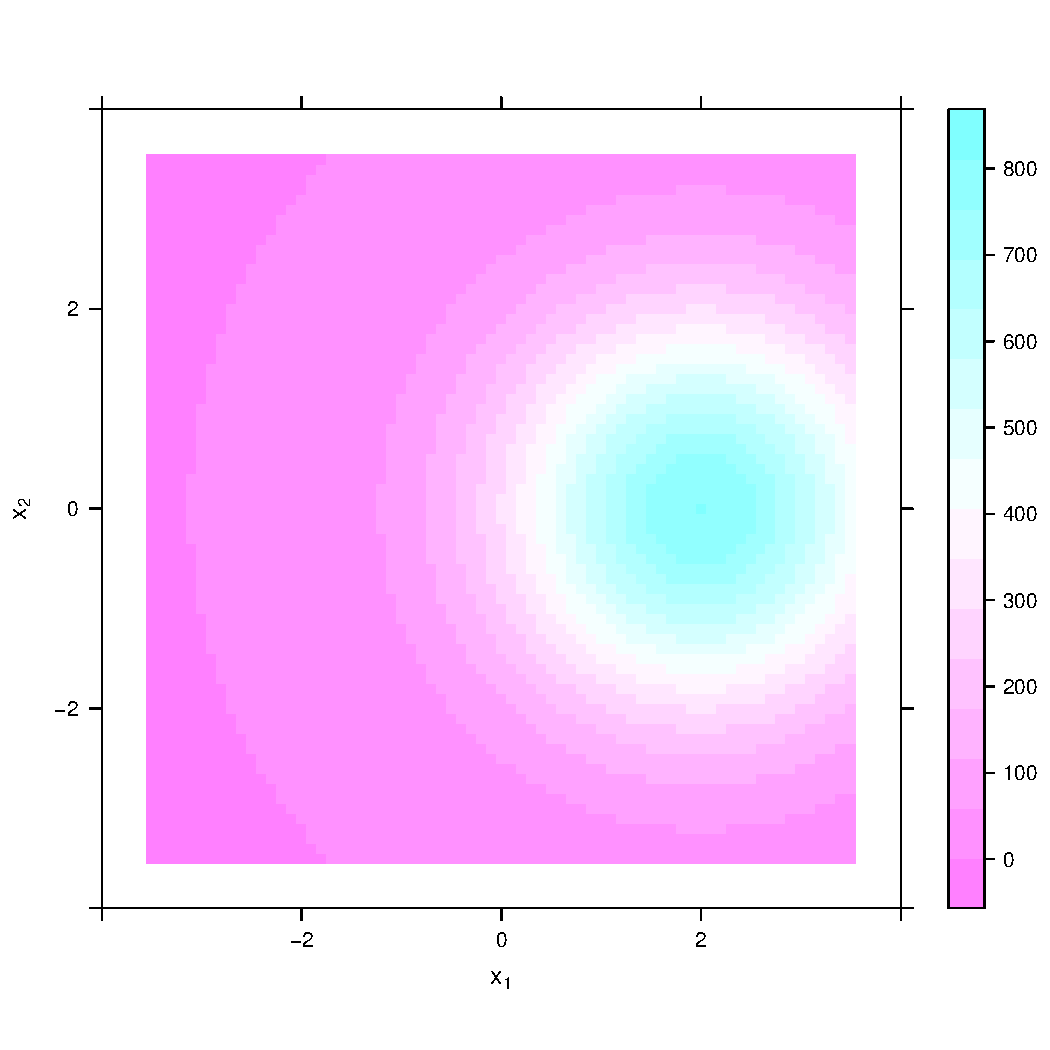
\includegraphics[width=\textwidth]{output/population-heatmap}
    \subcaption{Population distribution}
    \end{subfigure}
    \begin{subfigure}[t]{0.32\textwidth}
    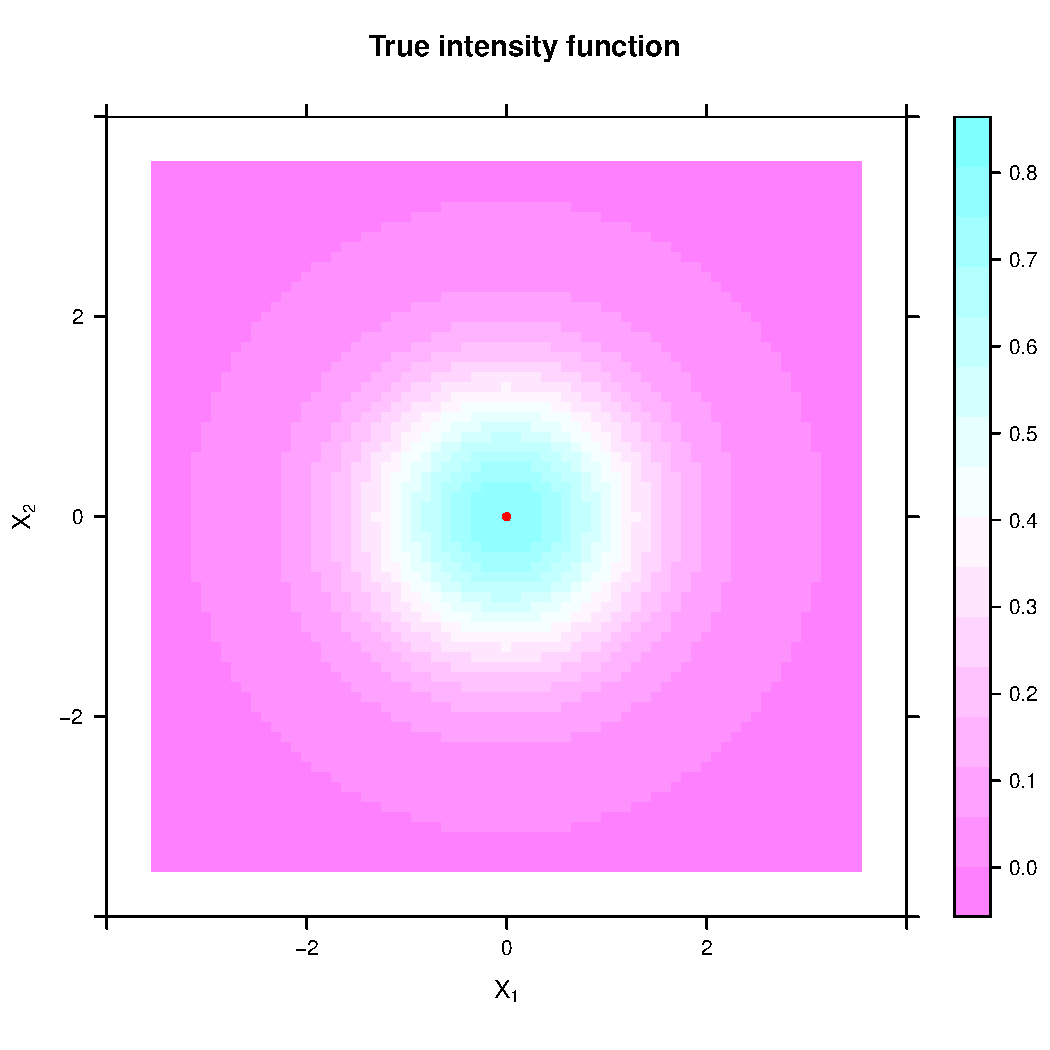
\includegraphics[width=\textwidth]{output/true_intensity_heatmap}
    \subcaption{True risk function}
    \end{subfigure}%
    \begin{subfigure}[t]{0.32\textwidth}
    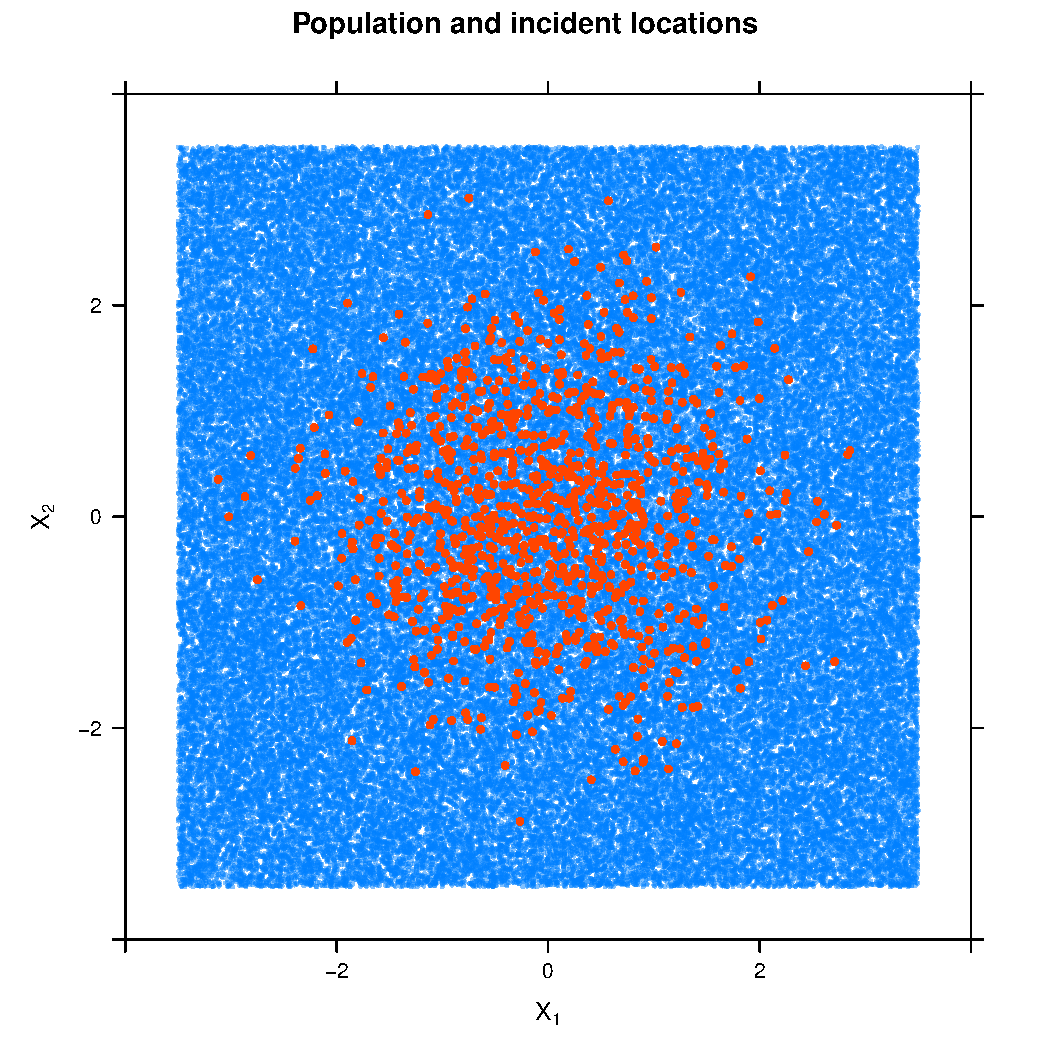
\includegraphics[width=\textwidth]{output/population_and_incidents_scatter}
    \subcaption{Population points (blue) with incidents (red)}
    \end{subfigure}%

    \caption[]{Population distribution (a), true risk function (b), and sample population with incidents (c) for uniform population of 10,000, uniform intensity of factor 100}
    \label{fig:distributions:unif_100_unif}    
\end{figure}


%%
%% Tables and figures for uniform population of 10,000, uniform intensity of factor 200
%%
\graphicspath{{./results/unif_200_unif/}}
\makeatletter
\def\input@path{{./results/unif_200_unif/}}
\makeatother

\begin{table}[H]
    \centering
    \scriptsize

    \begin{subtable}{0.5\textwidth}
    \subcaption{Means} 
    % latex table generated in R 3.3.3 by xtable 1.8-2 package
% Mon Jan 15 21:47:29 2018
\begin{tabular}{lrrr}
  \hline
 & Oracle & Silverman & CV \\ 
  \hline
MISE & 0.000022 & 0.000035 & 0.000033 \\ 
  Relative MISE & 0.003402 & 0.005404 & 0.004996 \\ 
  Normalized MISE & 0.000022 & 0.000035 & 0.000033 \\ 
  MIAE & 0.002515 & 0.003126 & 0.003003 \\ 
  Relative MIAE & 0.031137 & 0.038695 & 0.037178 \\ 
  Max Error & 0.021087 & 0.031111 & 0.029319 \\ 
  Peak bias & -0.010671 & 0.006739 & 0.004427 \\ 
  Relative Peak bias & -0.132093 & 0.083426 & 0.054803 \\ 
  Peak drift & 0.288634 & 0.418493 & 0.401299 \\ 
  Relative Peak drift & 0.041233 & 0.059785 & 0.057328 \\ 
  Centroid bias & -0.011216 & -0.000155 & -0.001331 \\ 
  Relative Centroid bias & -0.138849 & -0.001917 & -0.016472 \\ 
  Centroid drift & 0.207657 & 0.222708 & 0.221023 \\ 
  Relative Centroid drift & 0.029665 & 0.031815 & 0.031575 \\ 
   \hline
\end{tabular}

    \end{subtable}%
    \begin{subtable}{0.5\textwidth}
    \subcaption{Standard deviations} 
    % latex table generated in R 3.4.2 by xtable 1.8-2 package
% Thu Feb 15 19:57:40 2018
\begin{tabular}{lrrr}
  \hline
 & Oracle & Silverman & CV \\ 
  \hline
MISE & 0.000089 & 0.000116 & 0.000228 \\ 
  Relative MISE & 0.000131 & 0.000171 & 0.000335 \\ 
  Normalized MISE & 0.000018 & 0.000023 & 0.000046 \\ 
  MIAE & 0.000911 & 0.000820 & 0.001681 \\ 
  Relative MIAE & 0.001105 & 0.000994 & 0.002040 \\ 
  Max Error & 0.024919 & 0.036302 & 0.058950 \\ 
  Peak bias & 0.031372 & 0.045576 & 0.062499 \\ 
  Relative Peak bias & 0.038067 & 0.055302 & 0.075836 \\ 
  Peak drift & 0.060193 & 0.086240 & 0.111909 \\ 
  Relative Peak drift & 0.008599 & 0.012320 & 0.015987 \\ 
  Centroid bias & 0.031457 & 0.047196 & 0.046071 \\ 
  Relative Centroid bias & 0.038170 & 0.057267 & 0.055902 \\ 
  Centroid drift & 0.051758 & 0.054538 & 0.052729 \\ 
  Relative Centroid drift & 0.007394 & 0.007791 & 0.007533 \\ 
   \hline
\end{tabular}

    \end{subtable}

\caption[]{Error rates for uniform population of 10,000, uniform intensity of factor 200}
\label{tbl:mean_error_rates:unif_200_unif}
\end{table}

\begin{figure}[H]
        \centering
    \begin{subfigure}[t]{0.32\textwidth}
    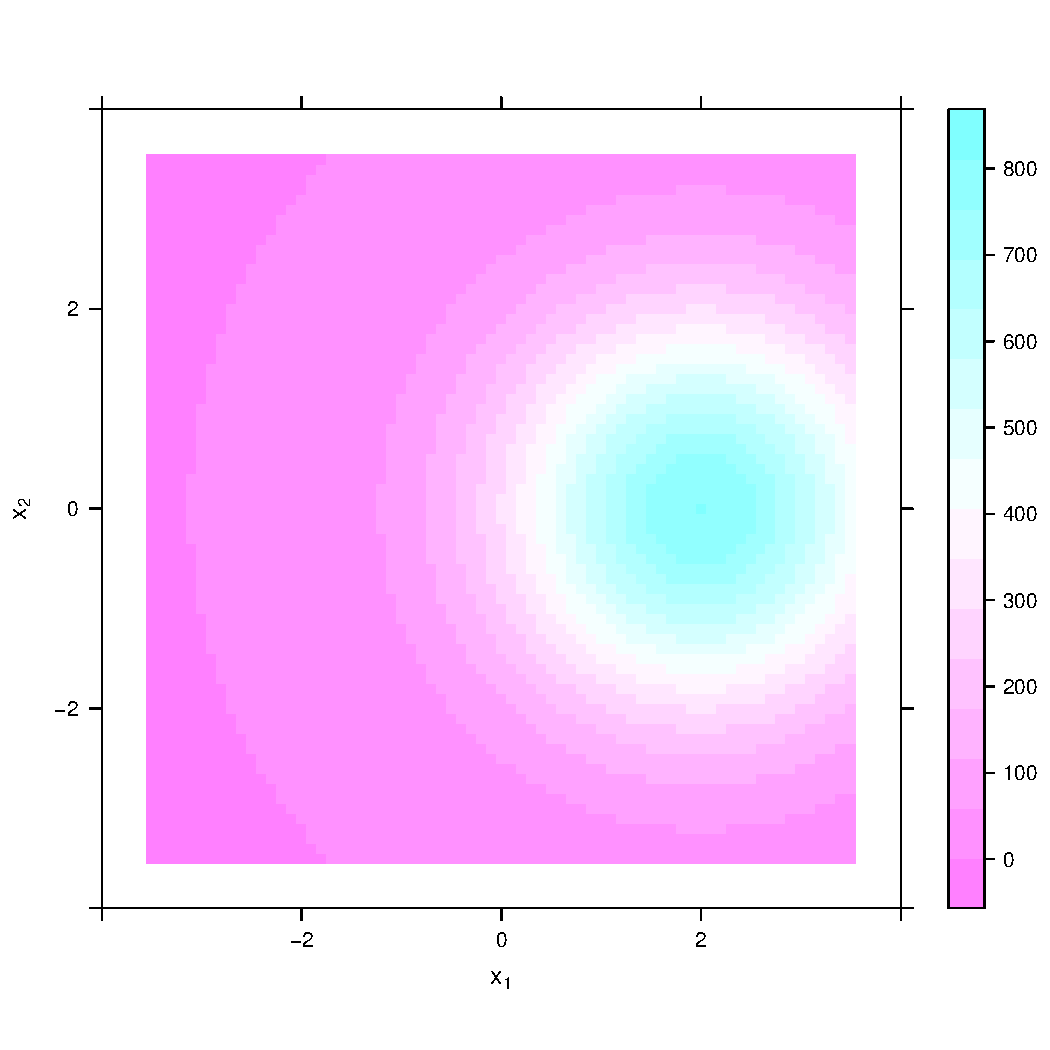
\includegraphics[width=\textwidth]{output/population-heatmap}
    \subcaption{Population distribution}
    \end{subfigure}
    \begin{subfigure}[t]{0.32\textwidth}
    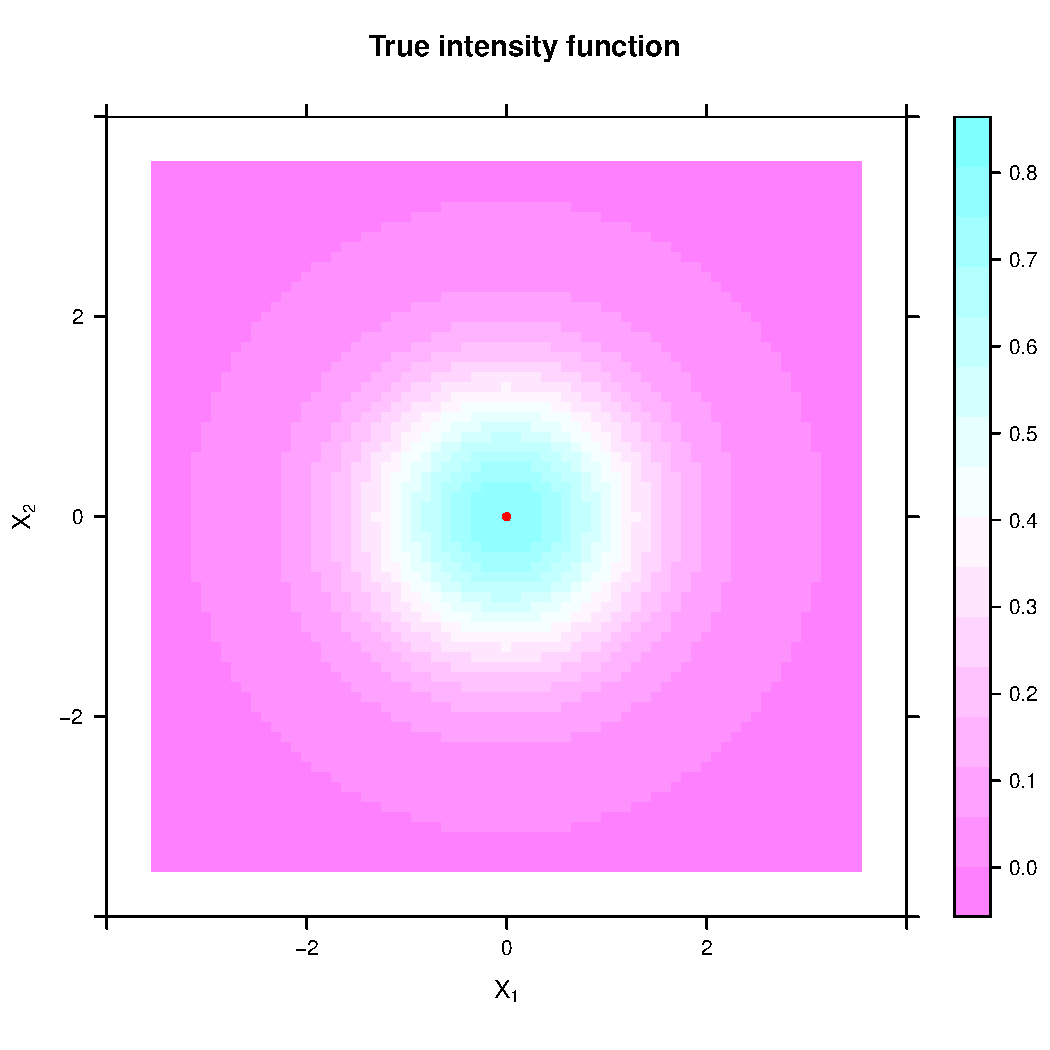
\includegraphics[width=\textwidth]{output/true_intensity_heatmap}
    \subcaption{True risk function}
    \end{subfigure}%
    \begin{subfigure}[t]{0.32\textwidth}
    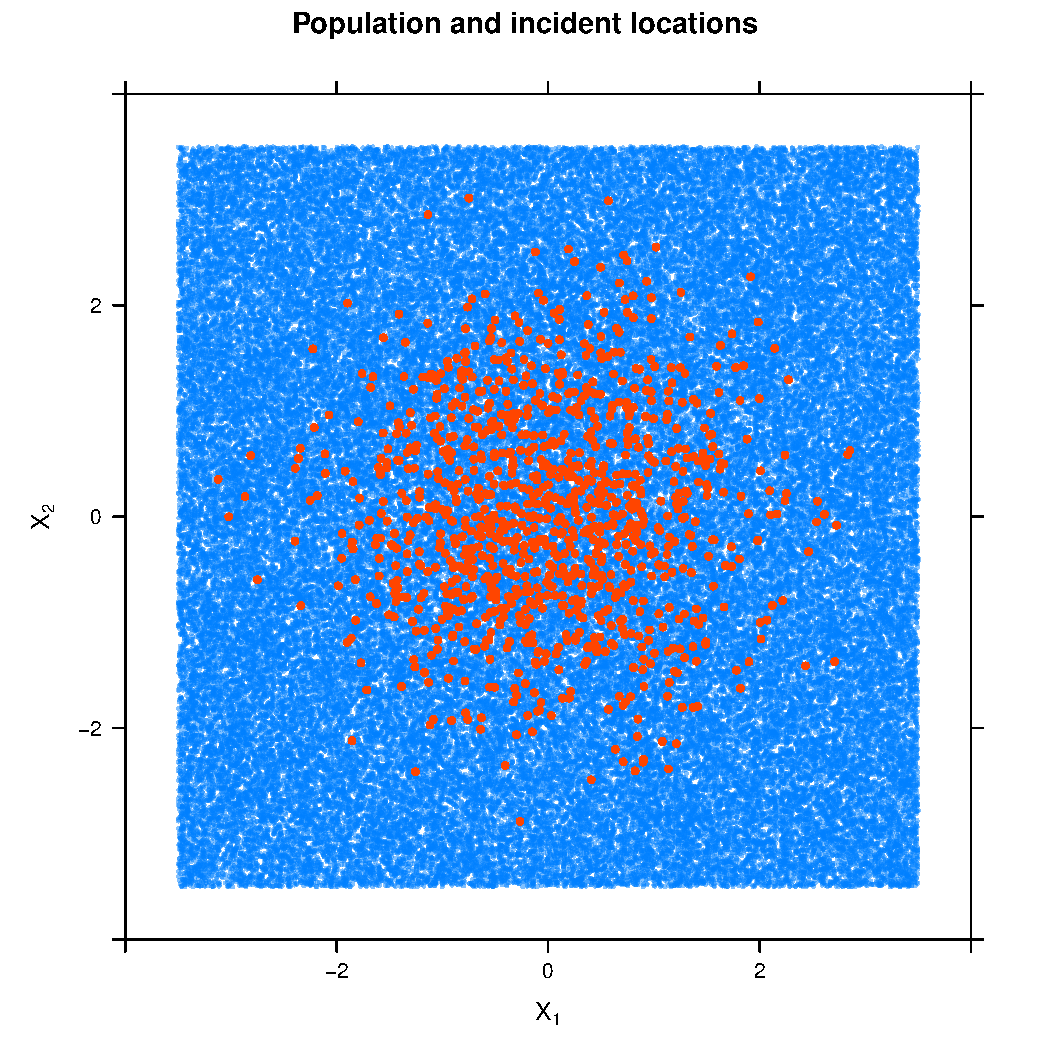
\includegraphics[width=\textwidth]{output/population_and_incidents_scatter}
    \subcaption{Population points (blue) with incidents (red)}
    \end{subfigure}%

    \caption[]{Population distribution (a), true risk function (b), and sample population with incidents (c) for uniform population of 10,000, uniform intensity of factor 200}
    \label{fig:distributions:unif_200_unif}    
\end{figure}


%%
%% Tables and figures for uniform population of 10,000, uniform intensity of factor 500
%%
\graphicspath{{./results/unif_500_unif/}}
\makeatletter
\def\input@path{{./results/unif_500_unif/}}
\makeatother

\begin{table}[H]
    \centering
    \scriptsize

    \begin{subtable}{0.5\textwidth}
    \subcaption{Means} 
    % latex table generated in R 3.3.3 by xtable 1.8-2 package
% Mon Jan 15 21:47:29 2018
\begin{tabular}{lrrr}
  \hline
 & Oracle & Silverman & CV \\ 
  \hline
MISE & 0.000022 & 0.000035 & 0.000033 \\ 
  Relative MISE & 0.003402 & 0.005404 & 0.004996 \\ 
  Normalized MISE & 0.000022 & 0.000035 & 0.000033 \\ 
  MIAE & 0.002515 & 0.003126 & 0.003003 \\ 
  Relative MIAE & 0.031137 & 0.038695 & 0.037178 \\ 
  Max Error & 0.021087 & 0.031111 & 0.029319 \\ 
  Peak bias & -0.010671 & 0.006739 & 0.004427 \\ 
  Relative Peak bias & -0.132093 & 0.083426 & 0.054803 \\ 
  Peak drift & 0.288634 & 0.418493 & 0.401299 \\ 
  Relative Peak drift & 0.041233 & 0.059785 & 0.057328 \\ 
  Centroid bias & -0.011216 & -0.000155 & -0.001331 \\ 
  Relative Centroid bias & -0.138849 & -0.001917 & -0.016472 \\ 
  Centroid drift & 0.207657 & 0.222708 & 0.221023 \\ 
  Relative Centroid drift & 0.029665 & 0.031815 & 0.031575 \\ 
   \hline
\end{tabular}

    \end{subtable}%
    \begin{subtable}{0.5\textwidth}
    \subcaption{Standard deviations} 
    % latex table generated in R 3.4.2 by xtable 1.8-2 package
% Thu Feb 15 19:57:40 2018
\begin{tabular}{lrrr}
  \hline
 & Oracle & Silverman & CV \\ 
  \hline
MISE & 0.000089 & 0.000116 & 0.000228 \\ 
  Relative MISE & 0.000131 & 0.000171 & 0.000335 \\ 
  Normalized MISE & 0.000018 & 0.000023 & 0.000046 \\ 
  MIAE & 0.000911 & 0.000820 & 0.001681 \\ 
  Relative MIAE & 0.001105 & 0.000994 & 0.002040 \\ 
  Max Error & 0.024919 & 0.036302 & 0.058950 \\ 
  Peak bias & 0.031372 & 0.045576 & 0.062499 \\ 
  Relative Peak bias & 0.038067 & 0.055302 & 0.075836 \\ 
  Peak drift & 0.060193 & 0.086240 & 0.111909 \\ 
  Relative Peak drift & 0.008599 & 0.012320 & 0.015987 \\ 
  Centroid bias & 0.031457 & 0.047196 & 0.046071 \\ 
  Relative Centroid bias & 0.038170 & 0.057267 & 0.055902 \\ 
  Centroid drift & 0.051758 & 0.054538 & 0.052729 \\ 
  Relative Centroid drift & 0.007394 & 0.007791 & 0.007533 \\ 
   \hline
\end{tabular}

    \end{subtable}

\caption[]{Error rates for uniform population of 10,000, uniform intensity of factor 500}
\label{tbl:mean_error_rates:unif_500_unif}
\end{table}

\begin{figure}[H]
        \centering
    \begin{subfigure}[t]{0.32\textwidth}
    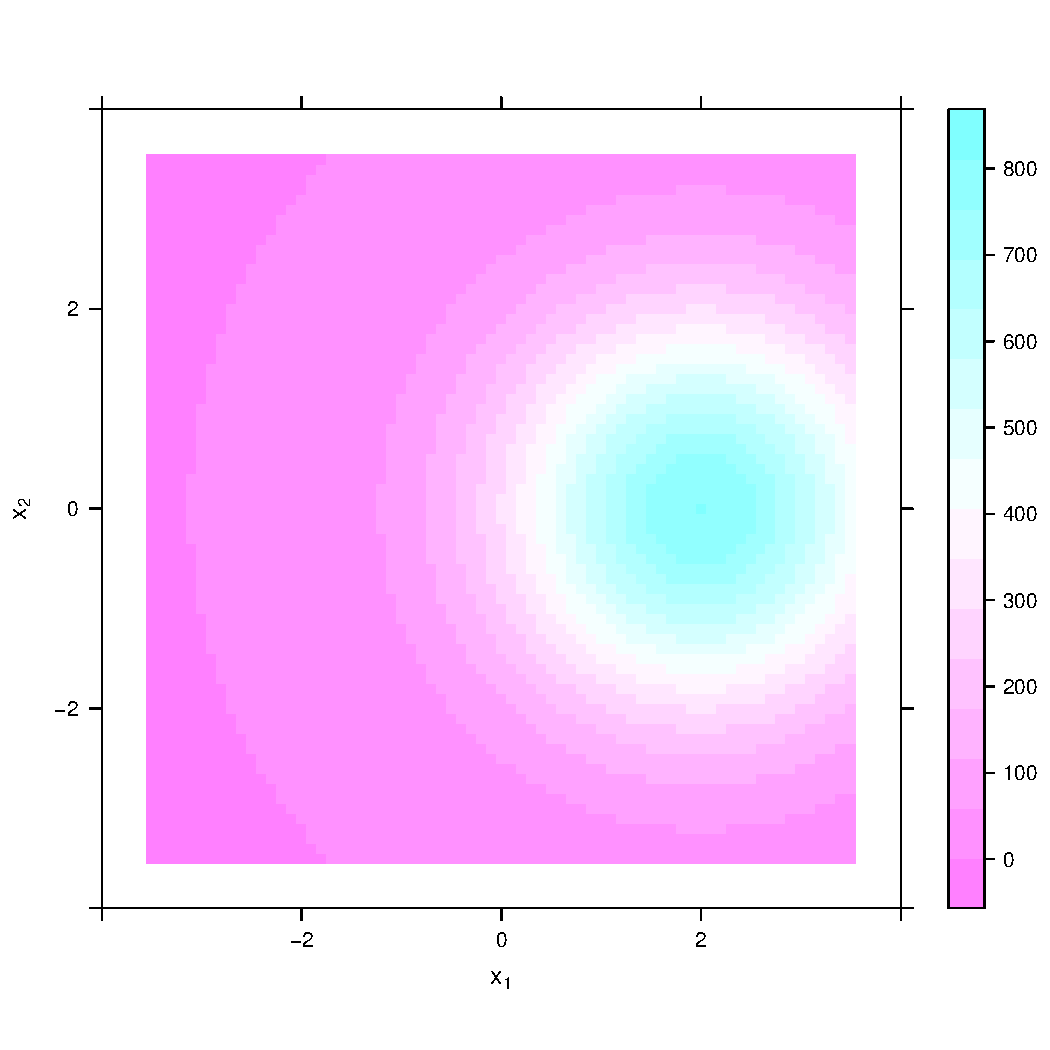
\includegraphics[width=\textwidth]{output/population-heatmap}
    \subcaption{Population distribution}
    \end{subfigure}
    \begin{subfigure}[t]{0.32\textwidth}
    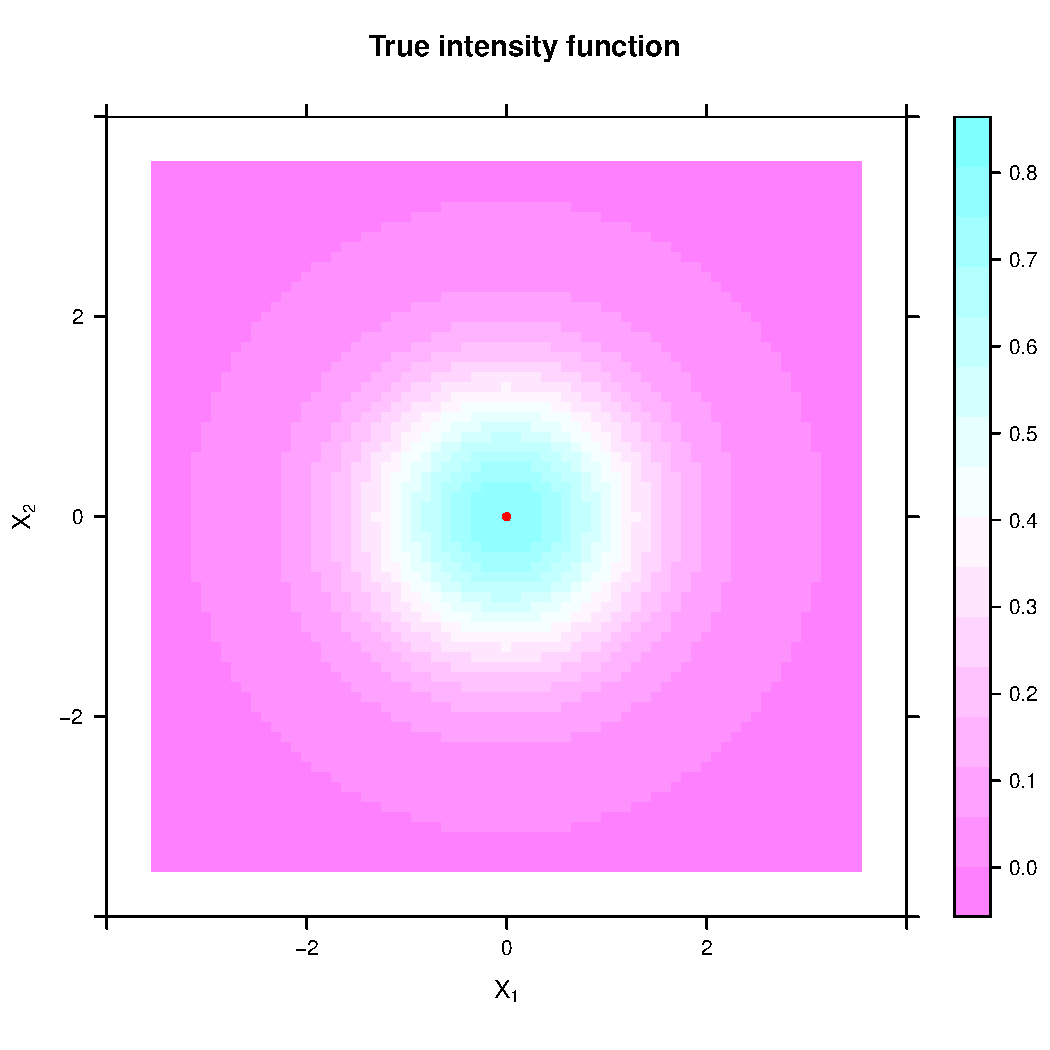
\includegraphics[width=\textwidth]{output/true_intensity_heatmap}
    \subcaption{True risk function}
    \end{subfigure}%
    \begin{subfigure}[t]{0.32\textwidth}
    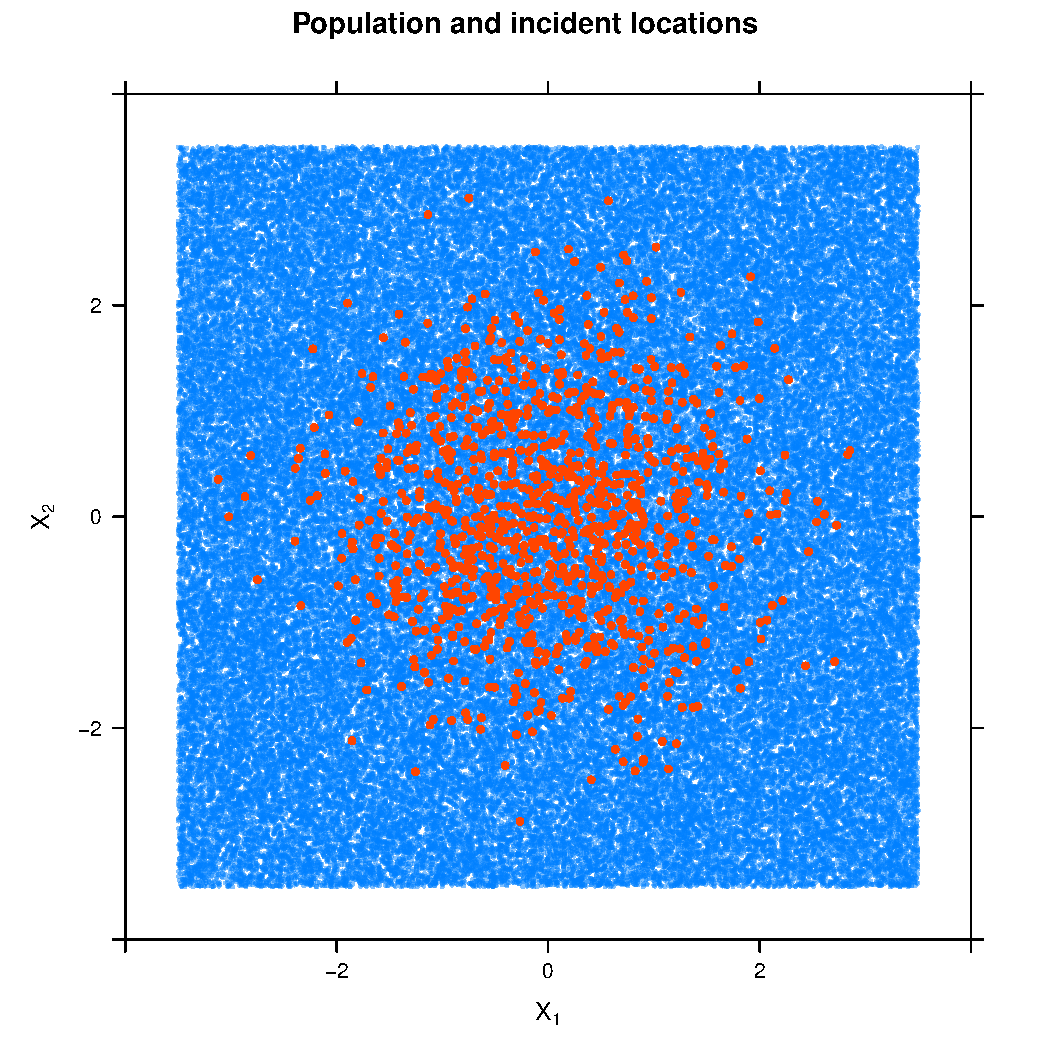
\includegraphics[width=\textwidth]{output/population_and_incidents_scatter}
    \subcaption{Population points (blue) with incidents (red)}
    \end{subfigure}%

    \caption[]{Population distribution (a), true risk function (b), and sample population with incidents (c) for uniform population of 10,000, uniform intensity of factor 500}
    \label{fig:distributions:unif_500_unif}    
\end{figure}


%%
%% Tables and figures for uniform population of 10,000, uniform intensity of factor 1,000
%%
\graphicspath{{./results/unif_1000_unif/}}
\makeatletter
\def\input@path{{./results/unif_1000_unif/}}
\makeatother

\begin{table}[H]
    \centering
    \scriptsize

    \begin{subtable}{0.5\textwidth}
    \subcaption{Means} 
    % latex table generated in R 3.3.3 by xtable 1.8-2 package
% Mon Jan 15 21:47:29 2018
\begin{tabular}{lrrr}
  \hline
 & Oracle & Silverman & CV \\ 
  \hline
MISE & 0.000022 & 0.000035 & 0.000033 \\ 
  Relative MISE & 0.003402 & 0.005404 & 0.004996 \\ 
  Normalized MISE & 0.000022 & 0.000035 & 0.000033 \\ 
  MIAE & 0.002515 & 0.003126 & 0.003003 \\ 
  Relative MIAE & 0.031137 & 0.038695 & 0.037178 \\ 
  Max Error & 0.021087 & 0.031111 & 0.029319 \\ 
  Peak bias & -0.010671 & 0.006739 & 0.004427 \\ 
  Relative Peak bias & -0.132093 & 0.083426 & 0.054803 \\ 
  Peak drift & 0.288634 & 0.418493 & 0.401299 \\ 
  Relative Peak drift & 0.041233 & 0.059785 & 0.057328 \\ 
  Centroid bias & -0.011216 & -0.000155 & -0.001331 \\ 
  Relative Centroid bias & -0.138849 & -0.001917 & -0.016472 \\ 
  Centroid drift & 0.207657 & 0.222708 & 0.221023 \\ 
  Relative Centroid drift & 0.029665 & 0.031815 & 0.031575 \\ 
   \hline
\end{tabular}

    \end{subtable}%
    \begin{subtable}{0.5\textwidth}
    \subcaption{Standard deviations} 
    % latex table generated in R 3.4.2 by xtable 1.8-2 package
% Thu Feb 15 19:57:40 2018
\begin{tabular}{lrrr}
  \hline
 & Oracle & Silverman & CV \\ 
  \hline
MISE & 0.000089 & 0.000116 & 0.000228 \\ 
  Relative MISE & 0.000131 & 0.000171 & 0.000335 \\ 
  Normalized MISE & 0.000018 & 0.000023 & 0.000046 \\ 
  MIAE & 0.000911 & 0.000820 & 0.001681 \\ 
  Relative MIAE & 0.001105 & 0.000994 & 0.002040 \\ 
  Max Error & 0.024919 & 0.036302 & 0.058950 \\ 
  Peak bias & 0.031372 & 0.045576 & 0.062499 \\ 
  Relative Peak bias & 0.038067 & 0.055302 & 0.075836 \\ 
  Peak drift & 0.060193 & 0.086240 & 0.111909 \\ 
  Relative Peak drift & 0.008599 & 0.012320 & 0.015987 \\ 
  Centroid bias & 0.031457 & 0.047196 & 0.046071 \\ 
  Relative Centroid bias & 0.038170 & 0.057267 & 0.055902 \\ 
  Centroid drift & 0.051758 & 0.054538 & 0.052729 \\ 
  Relative Centroid drift & 0.007394 & 0.007791 & 0.007533 \\ 
   \hline
\end{tabular}

    \end{subtable}

\caption[]{Error rates for uniform population of 10,000, uniform intensity of factor 1,000}
\label{tbl:mean_error_rates:unif_1000_unif}
\end{table}

\begin{figure}[H]
        \centering
    \begin{subfigure}[t]{0.32\textwidth}
    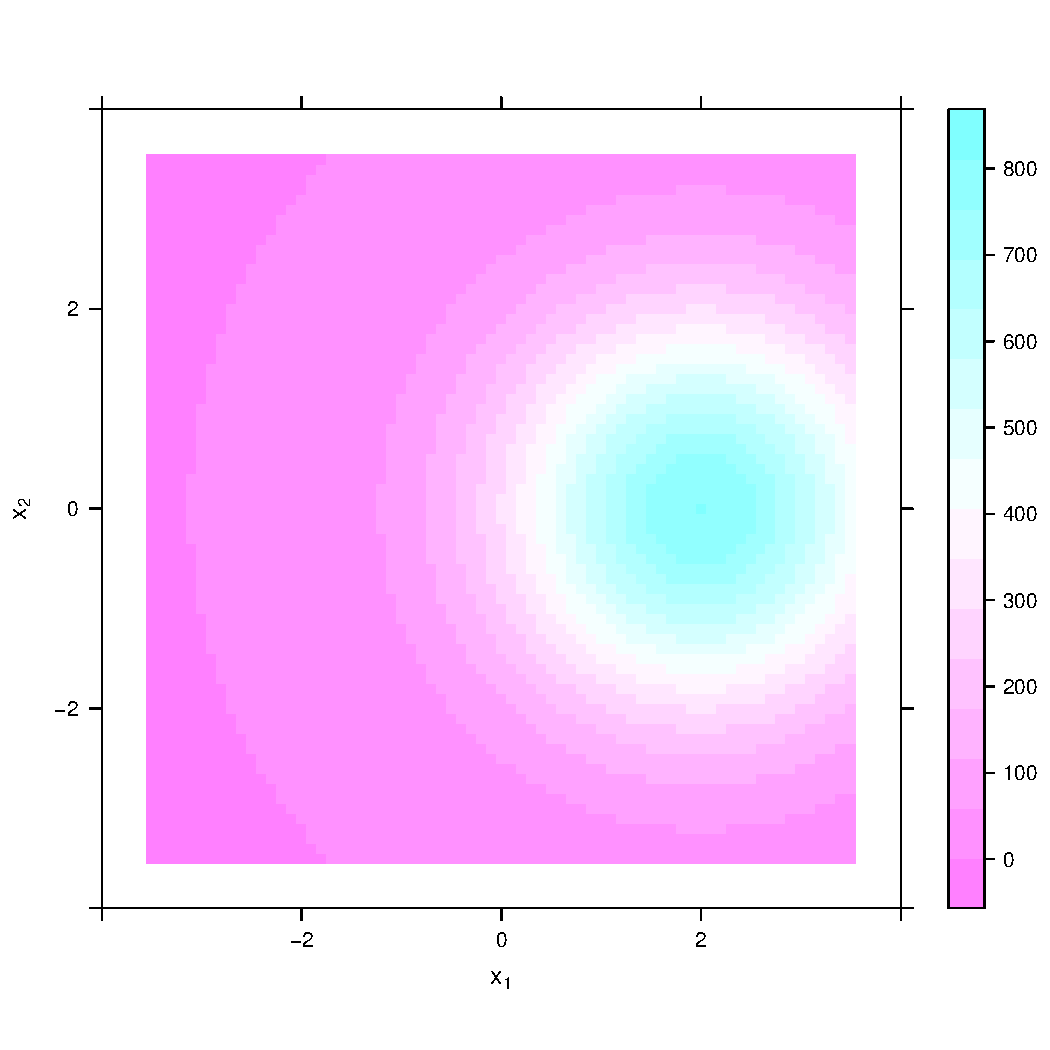
\includegraphics[width=\textwidth]{output/population-heatmap}
    \subcaption{Population distribution}
    \end{subfigure}
    \begin{subfigure}[t]{0.32\textwidth}
    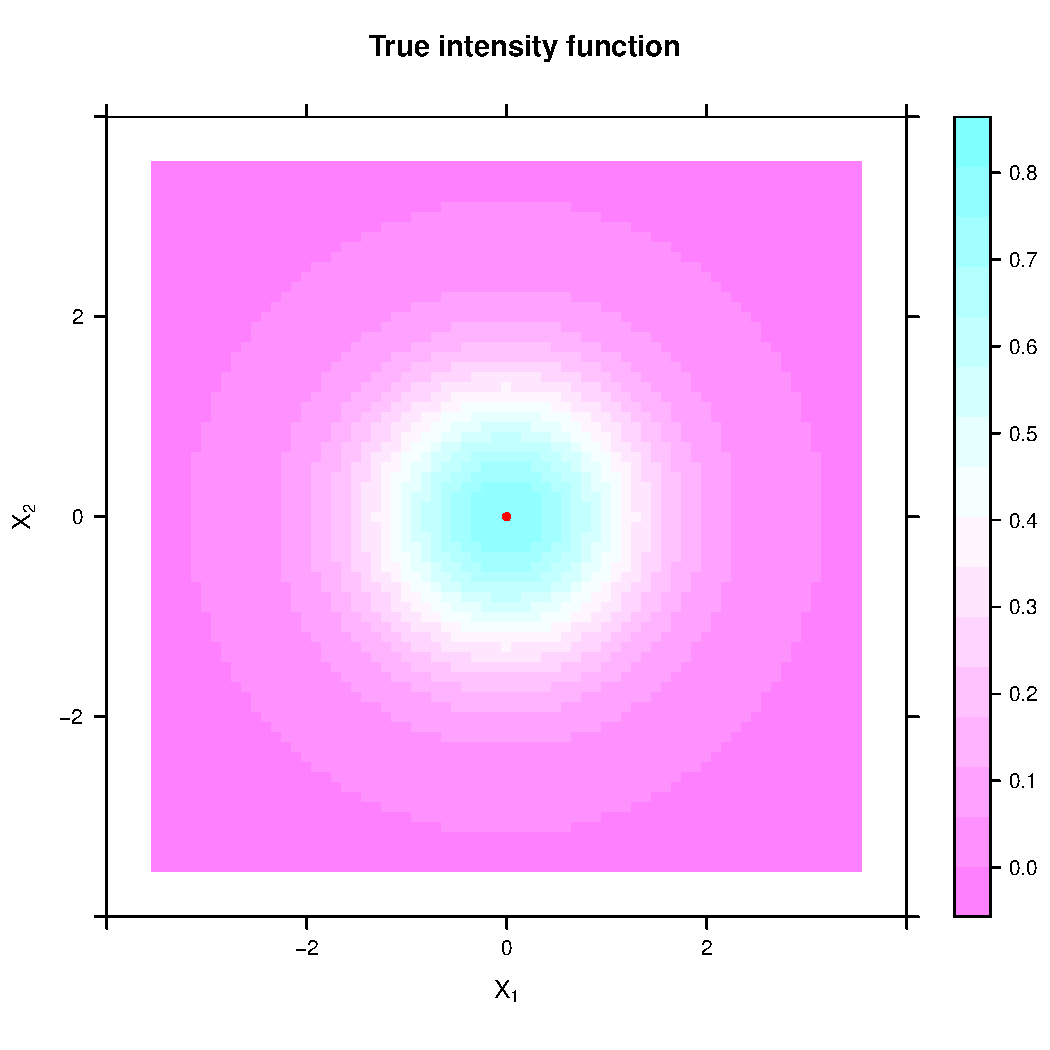
\includegraphics[width=\textwidth]{output/true_intensity_heatmap}
    \subcaption{True risk function}
    \end{subfigure}%
    \begin{subfigure}[t]{0.32\textwidth}
    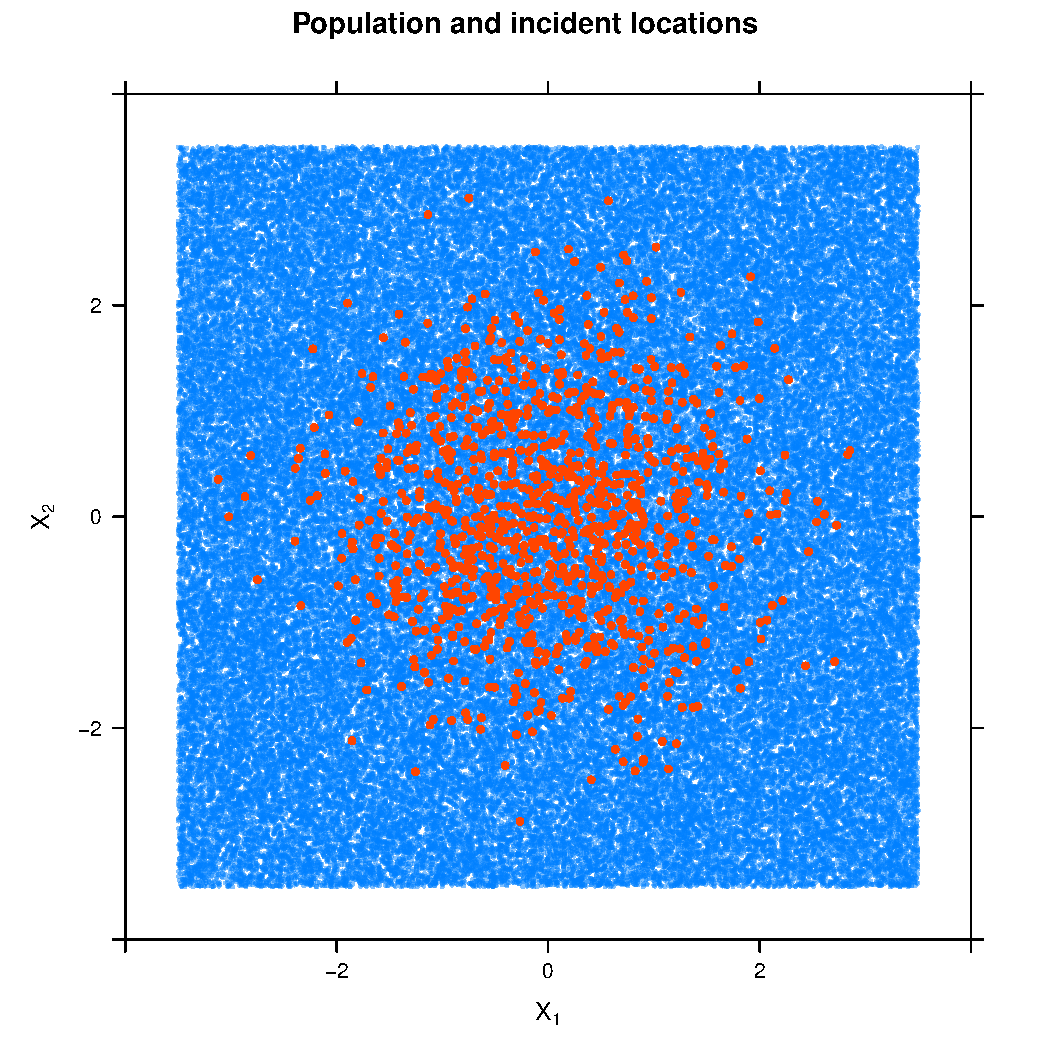
\includegraphics[width=\textwidth]{output/population_and_incidents_scatter}
    \subcaption{Population points (blue) with incidents (red)}
    \end{subfigure}%

    \caption[]{Population distribution (a), true risk function (b), and sample population with incidents (c) for uniform population of 10,000, uniform intensity of factor 1,000}
    \label{fig:distributions:unif_1000_unif}    
\end{figure}


    % unif100k_1000_1.0_1h
    % unif10k_100_1.0_1h
    % unif20k_200_1.0_1h
    % unif50k_500_1.0_1h
    % unif5k_50_1.0_1h
    % unif_1000_0.7_1h
    % unif_1000_1.0_1h
    % unif_1000_1.4_1h
    % unif_1000_2.0_1h
    % unif_1000_2.8_1h
    % unif_100_0.7_1h
    % unif_100_1.0_1h
    % unif_100_1.4_1h
    % unif_100_1_2h_1
    % unif_100_1_2h_2
    % unif_100_1_2h_3
    % unif_100_1_2h_4
    % unif_100_2.0_1h
    % unif_100_2.8_1h
    % unif_200_0.7_1h
    % unif_200_1.0_1h
    % unif_200_1.4_1h
    % unif_200_2.0_1h
    % unif_200_2.8_1h
    % unif_500_0.7_1h
    % unif_500_1.0_1h
    % unif_500_1.4_1h
    % unif_500_2.0_1h
    % unif_500_2.8_1h
    % unif_50_0.7_1h
    % unif_50_1.0_1h
    % unif_50_1.4_1h
    % unif_50_2.0_1h
    % unif_50_2.8_1h
    % p0.7_100_1.0_1h
    % p1.0_100_1.0_1h
    % p1.4_100_1.0_1h
    % p1.4_100_1_1h_1s
    % p1.4_100_1_1h_2s
    % p1.4_100_1_1h_3s
    % p1.4_100_1_1h_4s
    % p2.0_100_1.0_1h
    % p2.8_100_1.0_1h
